\section{Discussion} \label{sec:discussion}

In this paper, we have shown with detail the importance of accurately modelling the mixing details in the O-burning shell during an O-C shell merger.
We have demonstrated the importance of understanding the convective-reactive nature of the nucleosynthesis in the O-shell as material both advects and reacts. 
We show that $\gamma$-process nucleosynthesis is sensitive to the presence of a convective downturn and mixing speeds of that downturn in a way that is both non-linear and non-monotonic both globally and for specific isotopes, and that the ratio of isotopic pairs is found to be dependent on the mixing details. 
We also demonstrate why a O-C shell merger is necessary produce these isotopes in a pre-explosive context and how the ingestion rate boosts production.
Similarly, we show how the presence of a dip in the diffusion profile with either a GOSH-like dip or partial merger decrease the production of p-nuclei and how the deeper location of the GOSH-like dip is more effective at lowering production.
Finally, we show how varying the input nuclear physics causes a spread in the production of the p-nuclei, but that the specific details of how much a particular isotope is affected by that depends on mixing scenario.
In addition, the reaction rates that are relevant for the production of the p-nuclei are found depend on the mixing scenario.
Figure \ref{fig:impact_mixing_cases_bars_all} shows the maximum and minimum impact to the production on the p-nuclei due to the various mixing scenarios and across all these cases the average spread is $2.45~\mathrm{dex}$.

\begin{figure}[!htbp]
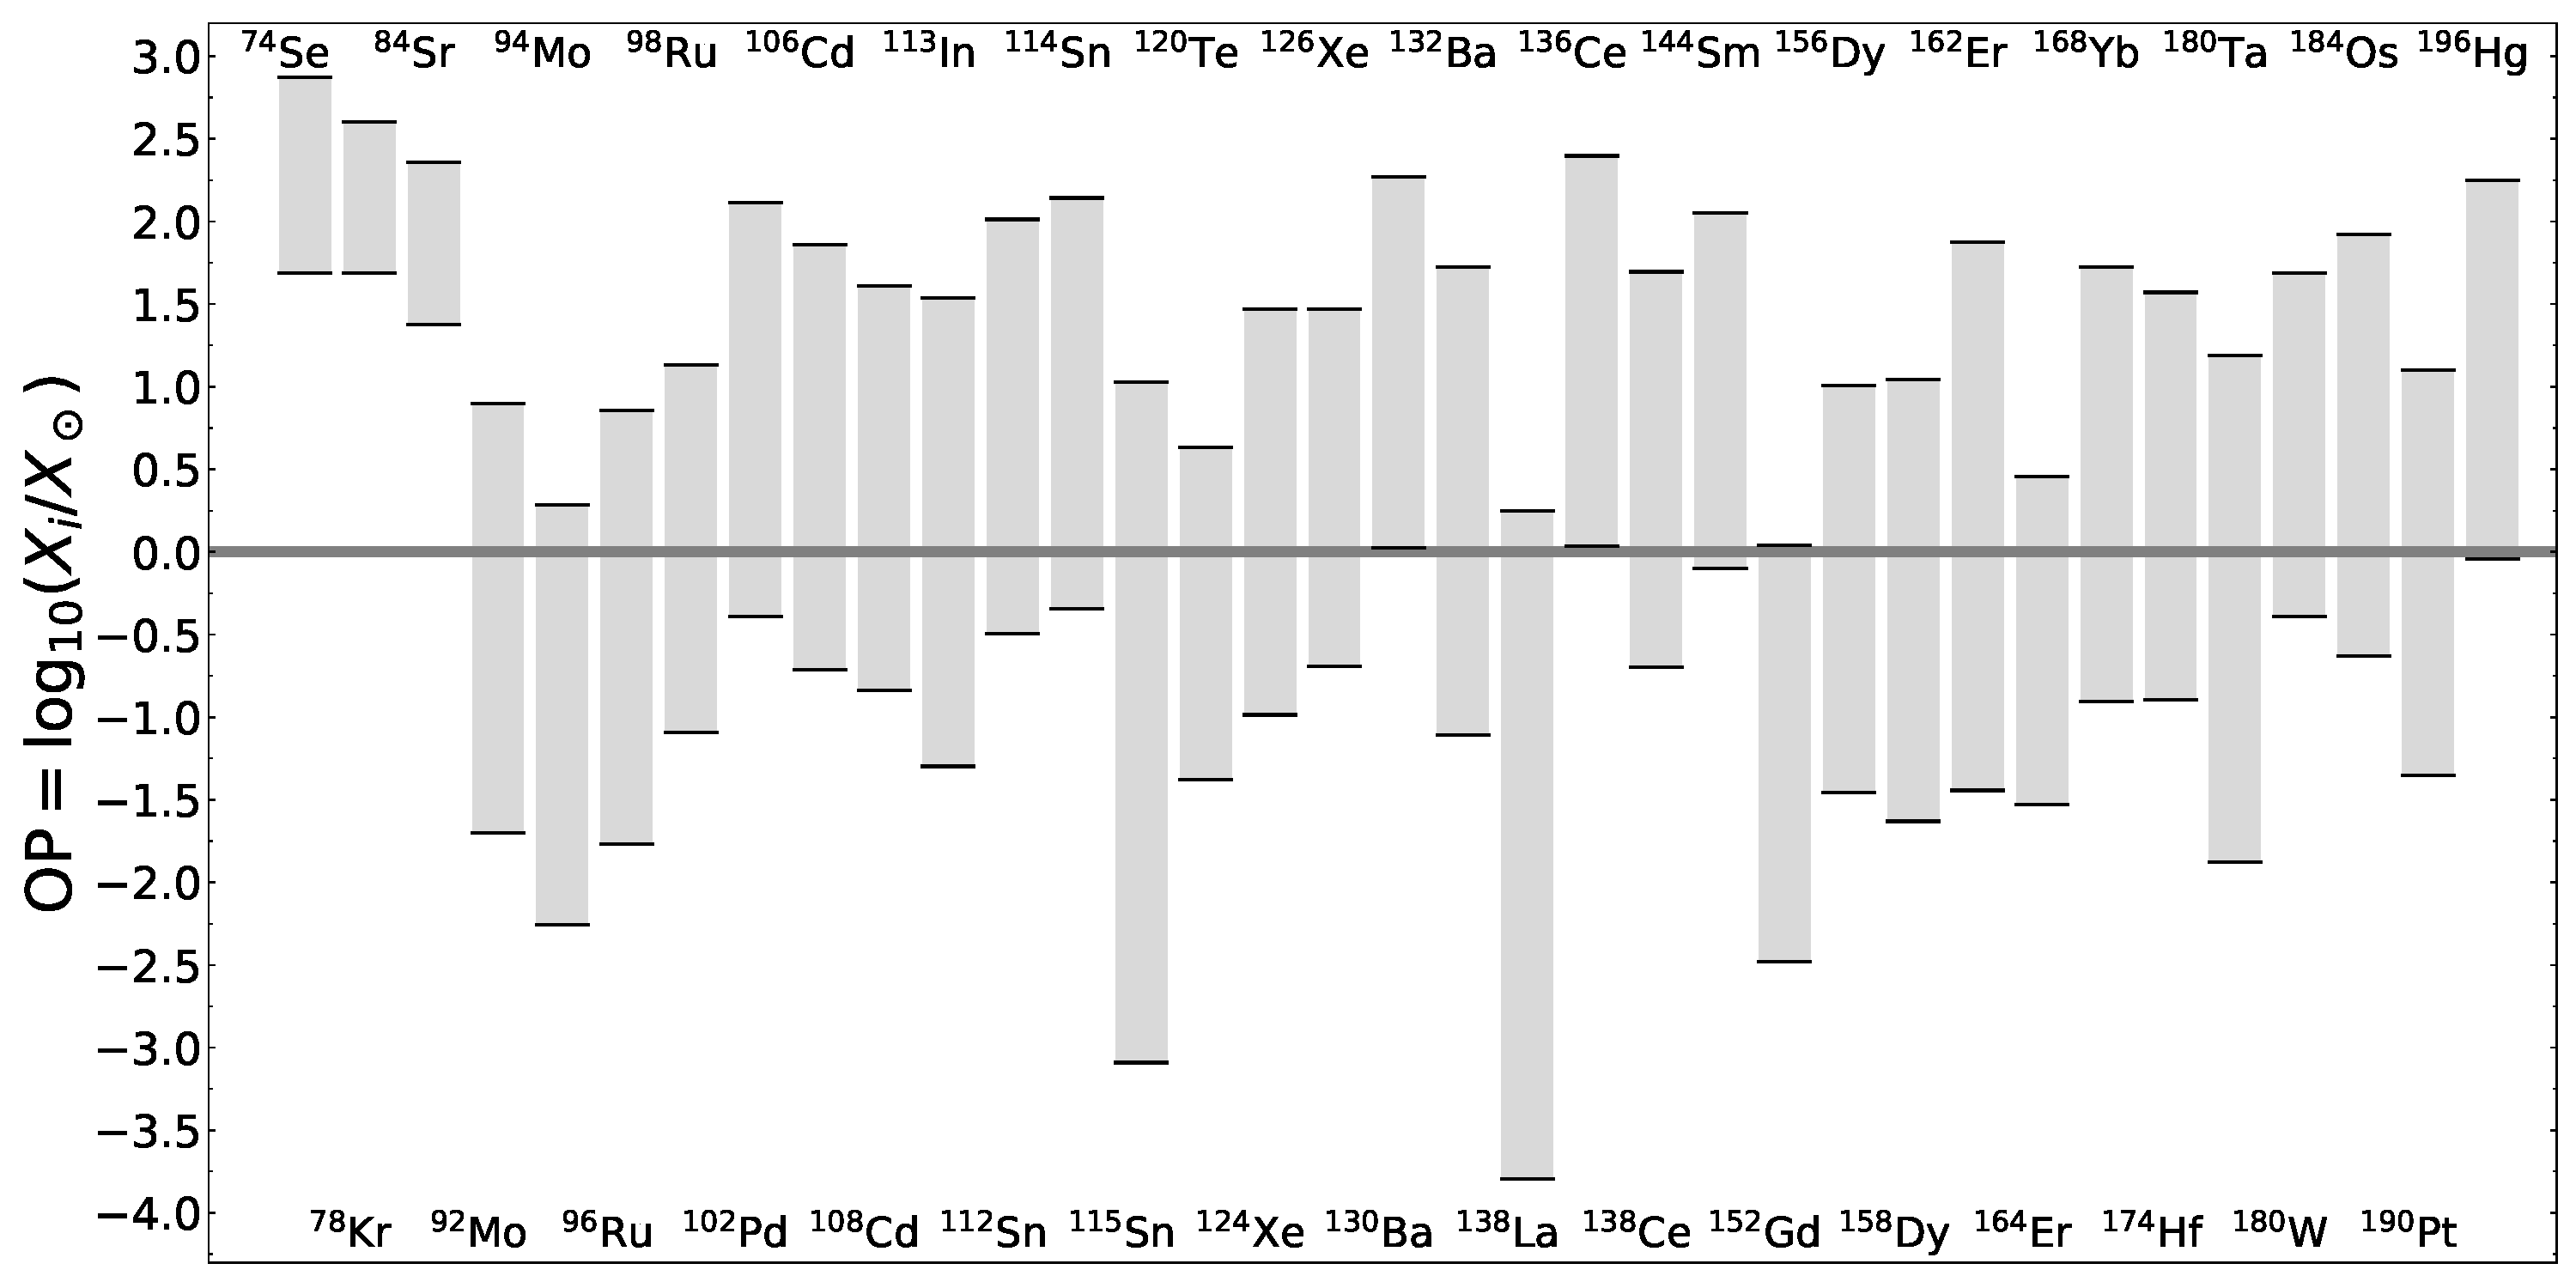
\includegraphics[width=\textwidth]{chapters/2/figures/impact_mixing_cases_bars_all.pdf}
\caption{Maximum and minimum overproduction compared to solar for all convective downturn scenarios, GOSH-like scenarios, partial merger scenarios, and ingestion rates excluding the scenario of no C-shell ingestion. The thick grey line at $\mathrm{OP}=0$ corresponds to the solar measurement. The average spread in production is $2.45~\mathrm{dex}$.
\label{fig:impact_mixing_cases_bars_all}}
\end{figure}

These results have a similar variation in final production for the p-nuclei as found by \cite{rauscherUncertaintiesProductionNuclei2016} when determining the uncertainties from nuclear physics inputs.
The $15M_\odot$ KEPLER model they analyze had an average uncertainity of $0.61$ for the $90\%$ probability from varying of the nuclear physics.
This is lower than this study which finds an average maximum spread of $3.6-6.2$ depending on the mixing case, but it is comparing $90\%$ probability to maximum.
They also find key rates correlated with the production of p-nuclei, of which some are shared in this study and others are not.

This work raises the importance of considering the limitations of mixing length theory for the nucleosynthesis of this 3-D hydrodynamic effect.
As shown by \cite{rizzutiShellMergersLate2024a} the nucleosynthesis in 3-D simulations does not match 1-D.
There remains more work to be done in analyzing the unique nucleosynthesis during O-C shell mergers and its greater relevance to observations and galatic chemical evolution (GCE) both for the p-nuclei and beyond. 
\cite{ritterConvectivereactiveNucleosynthesisSc2018} found in analyzing this model that there was an enhancement in the production of $^{31}\mathrm{P}$, $^{35}\mathrm{Cl}$, $^{39}\mathrm{K}$, and $^{45}\mathrm{Sc}$ during the O-C shell merger which could account for their underproduction in GCE models.
This has been confirmed to be a robust result across metallicity and stellar evolution model as shown by \cite{robertiOccurrenceImpactCarbonOxygen2025}.
Recent observations have found $\mathrm{P}$-enhanced stars \citep{masseronPhosphorusrichStarsUnusual2020, braunerUnveilingChemicalFingerprint2023, braunerUnveilingChemicalFingerprint2024} which could be explained by O-C shell merger, although this analysis has not been done.
There is also the general increase of O-burning ashes and decrease of C-shell ashes during the merger \citep{robertiOccurrenceImpactCarbonOxygen2025}, and if O-C shell mergers occurs in a  significant fraction of massive stars then there will be a noticable GCE impact.

There are also implications this work has on those interpretting the source of presolar grains. 
\cite{fokSiliconIsotopicComposition2024} argues that the nucleosynthesis in O-C shell mergers needs to be more closely analyzed because they matter when interpreting the $^{29}\mathrm{Si}/^{28}\mathrm{Si}$ ratio. 
As the mixing uncertainties show, there are more significant modelling concerns that need to be addressed when considering how O-C shell mergers may contribute presolar grains.
As shown in this work, the ratio of p-isotope pairs is sensitive to whether there is a convective downturn and the speed of the convective velocities in the O-shell.
Comparing measurements of meteorite grains data \citep{hynesPresolarGrainDatabase2009,stephanPresolarGrainDatabase2024a,stephanPresolarGrainDatabase2024} with the results from this paper, we find no single mixing scenario can explain isotopic grains data.
\begin{figure}[!htbp]
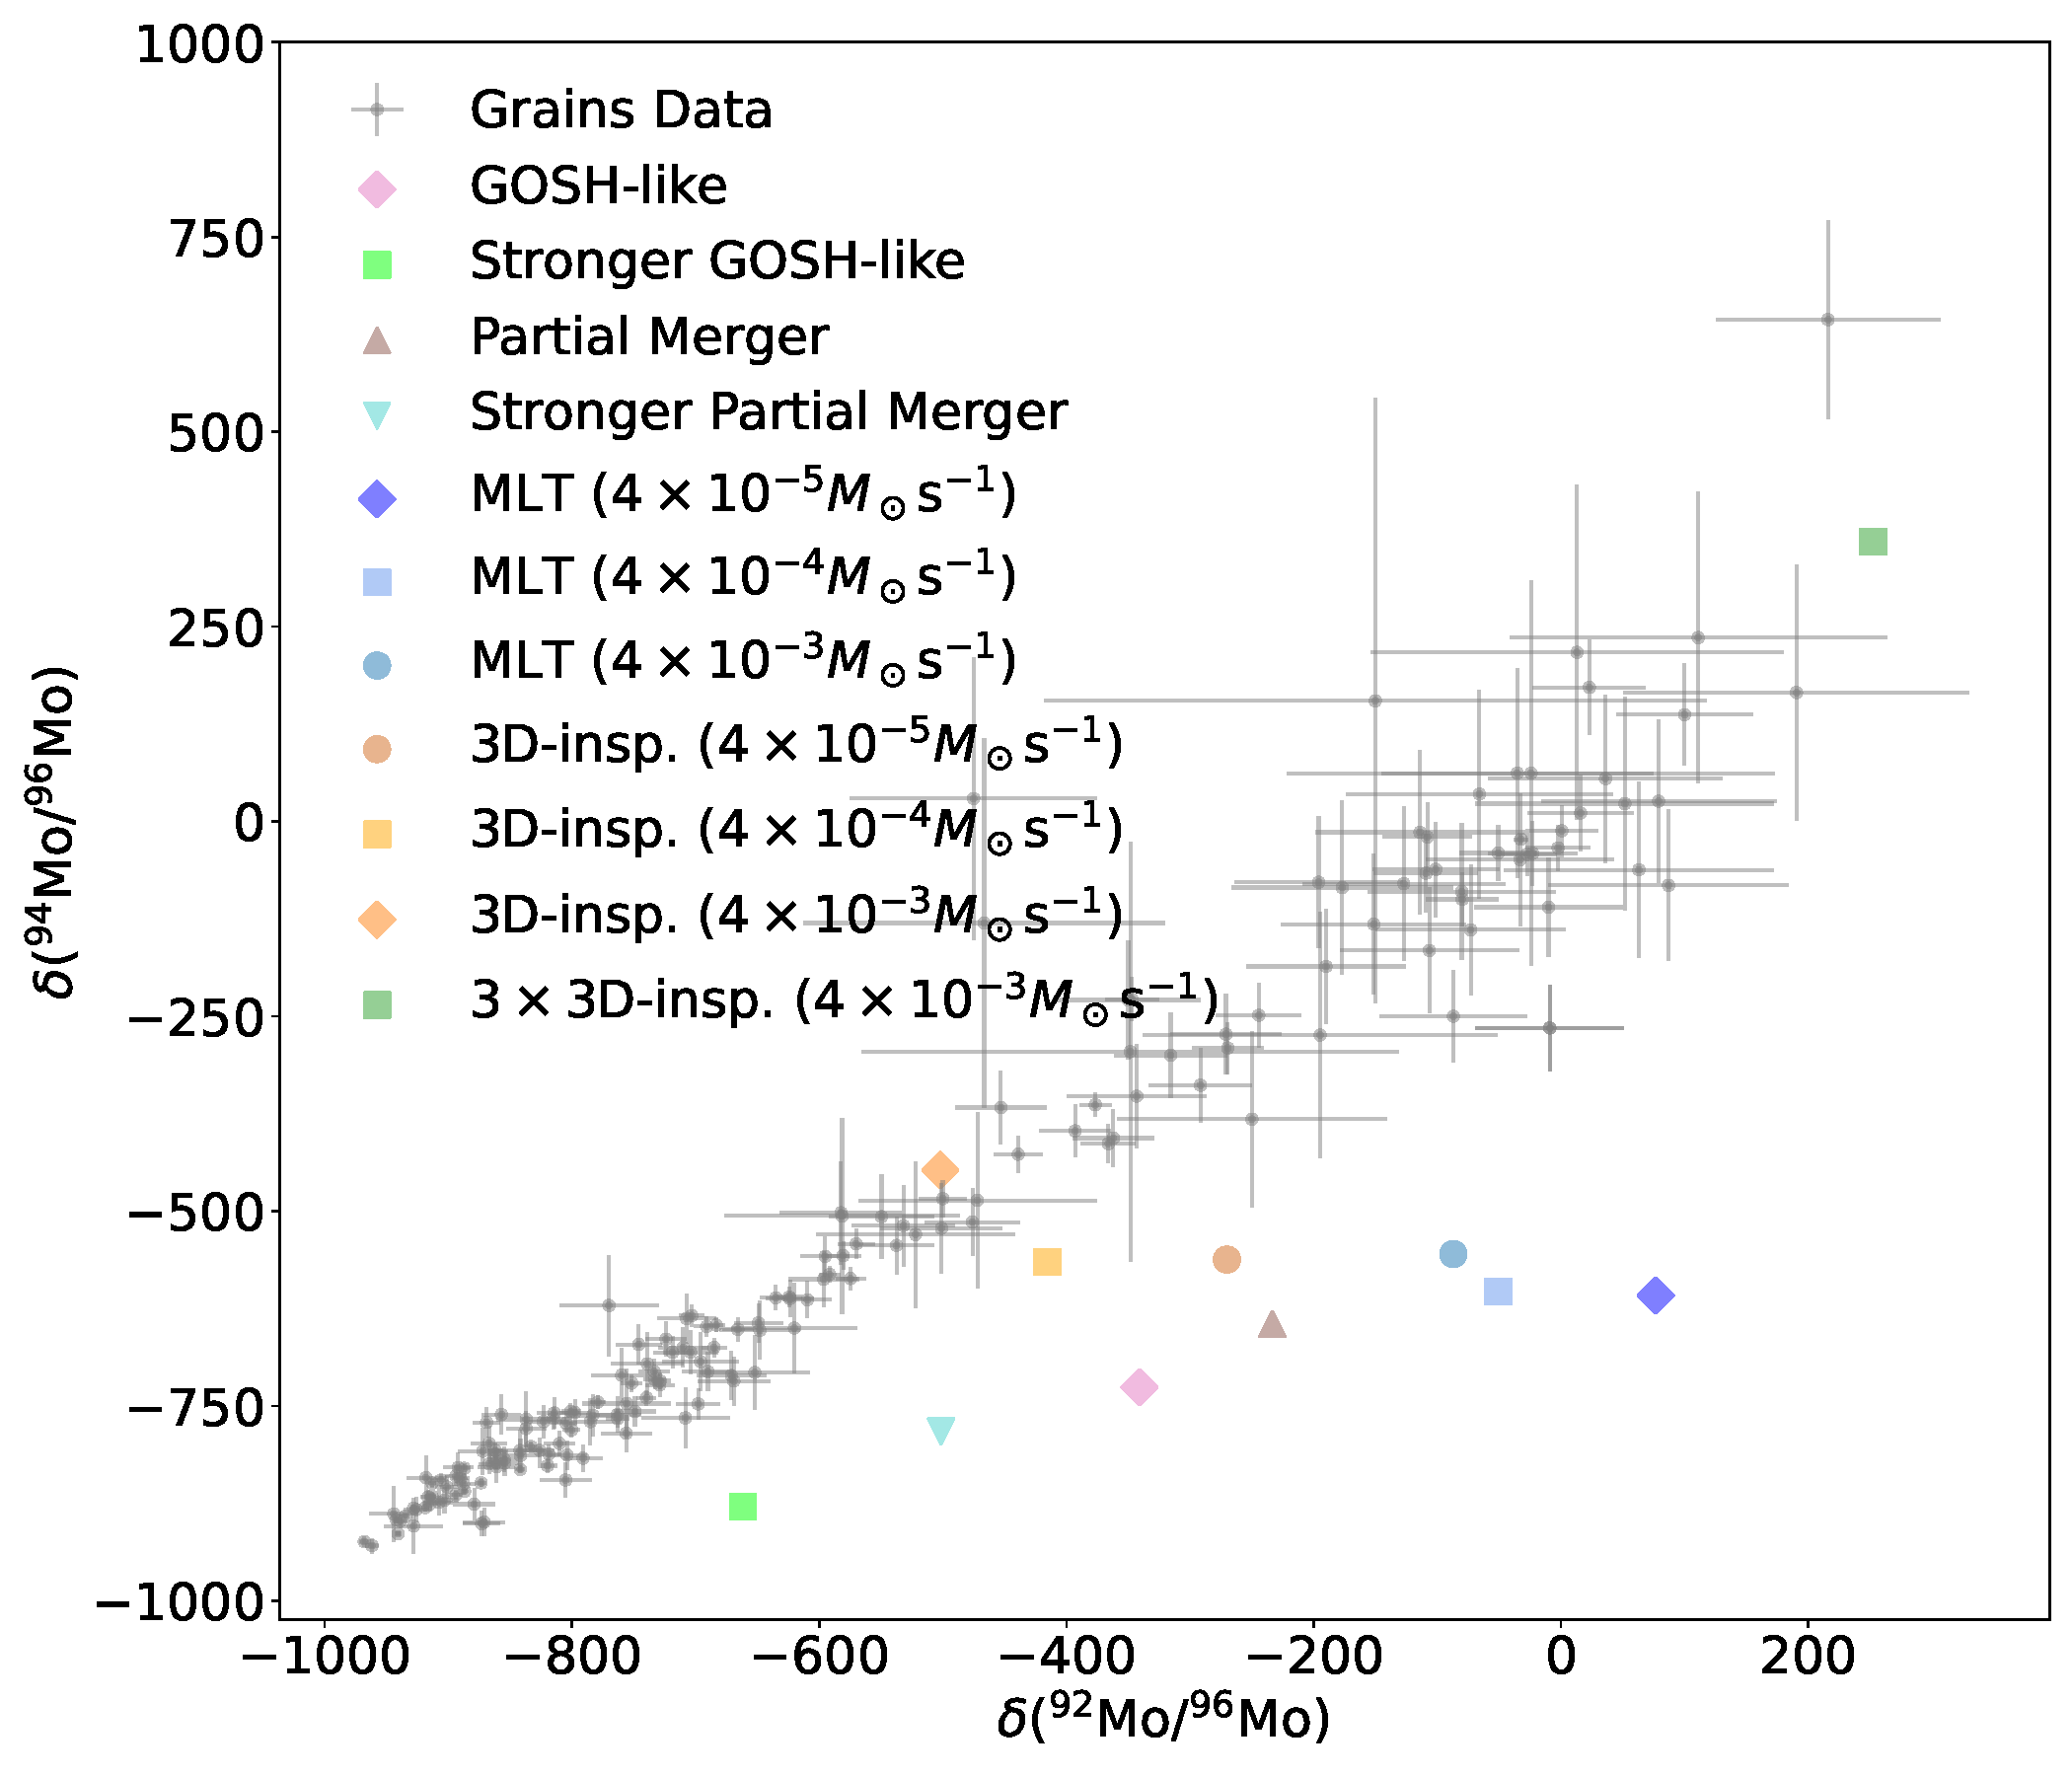
\includegraphics[width=\textwidth]{chapters/2/figures/grains_Mo92_Mo94_Mo96.pdf}
\caption{Comparing the results of the grains data to the various mixing scenarios considered in this paper for $\delta(^{92}\mathrm{Mo}/^{96}\mathrm{Mo})$ and $\delta(^{94}\mathrm{Mo}/^{96}\mathrm{Mo})$. Grey points correspond to grains data with $1\sigma$ error bars and coloured points for the mixing scenarios.
\label{fig:grains_Mo}}
\end{figure}
\begin{figure}[!htbp]
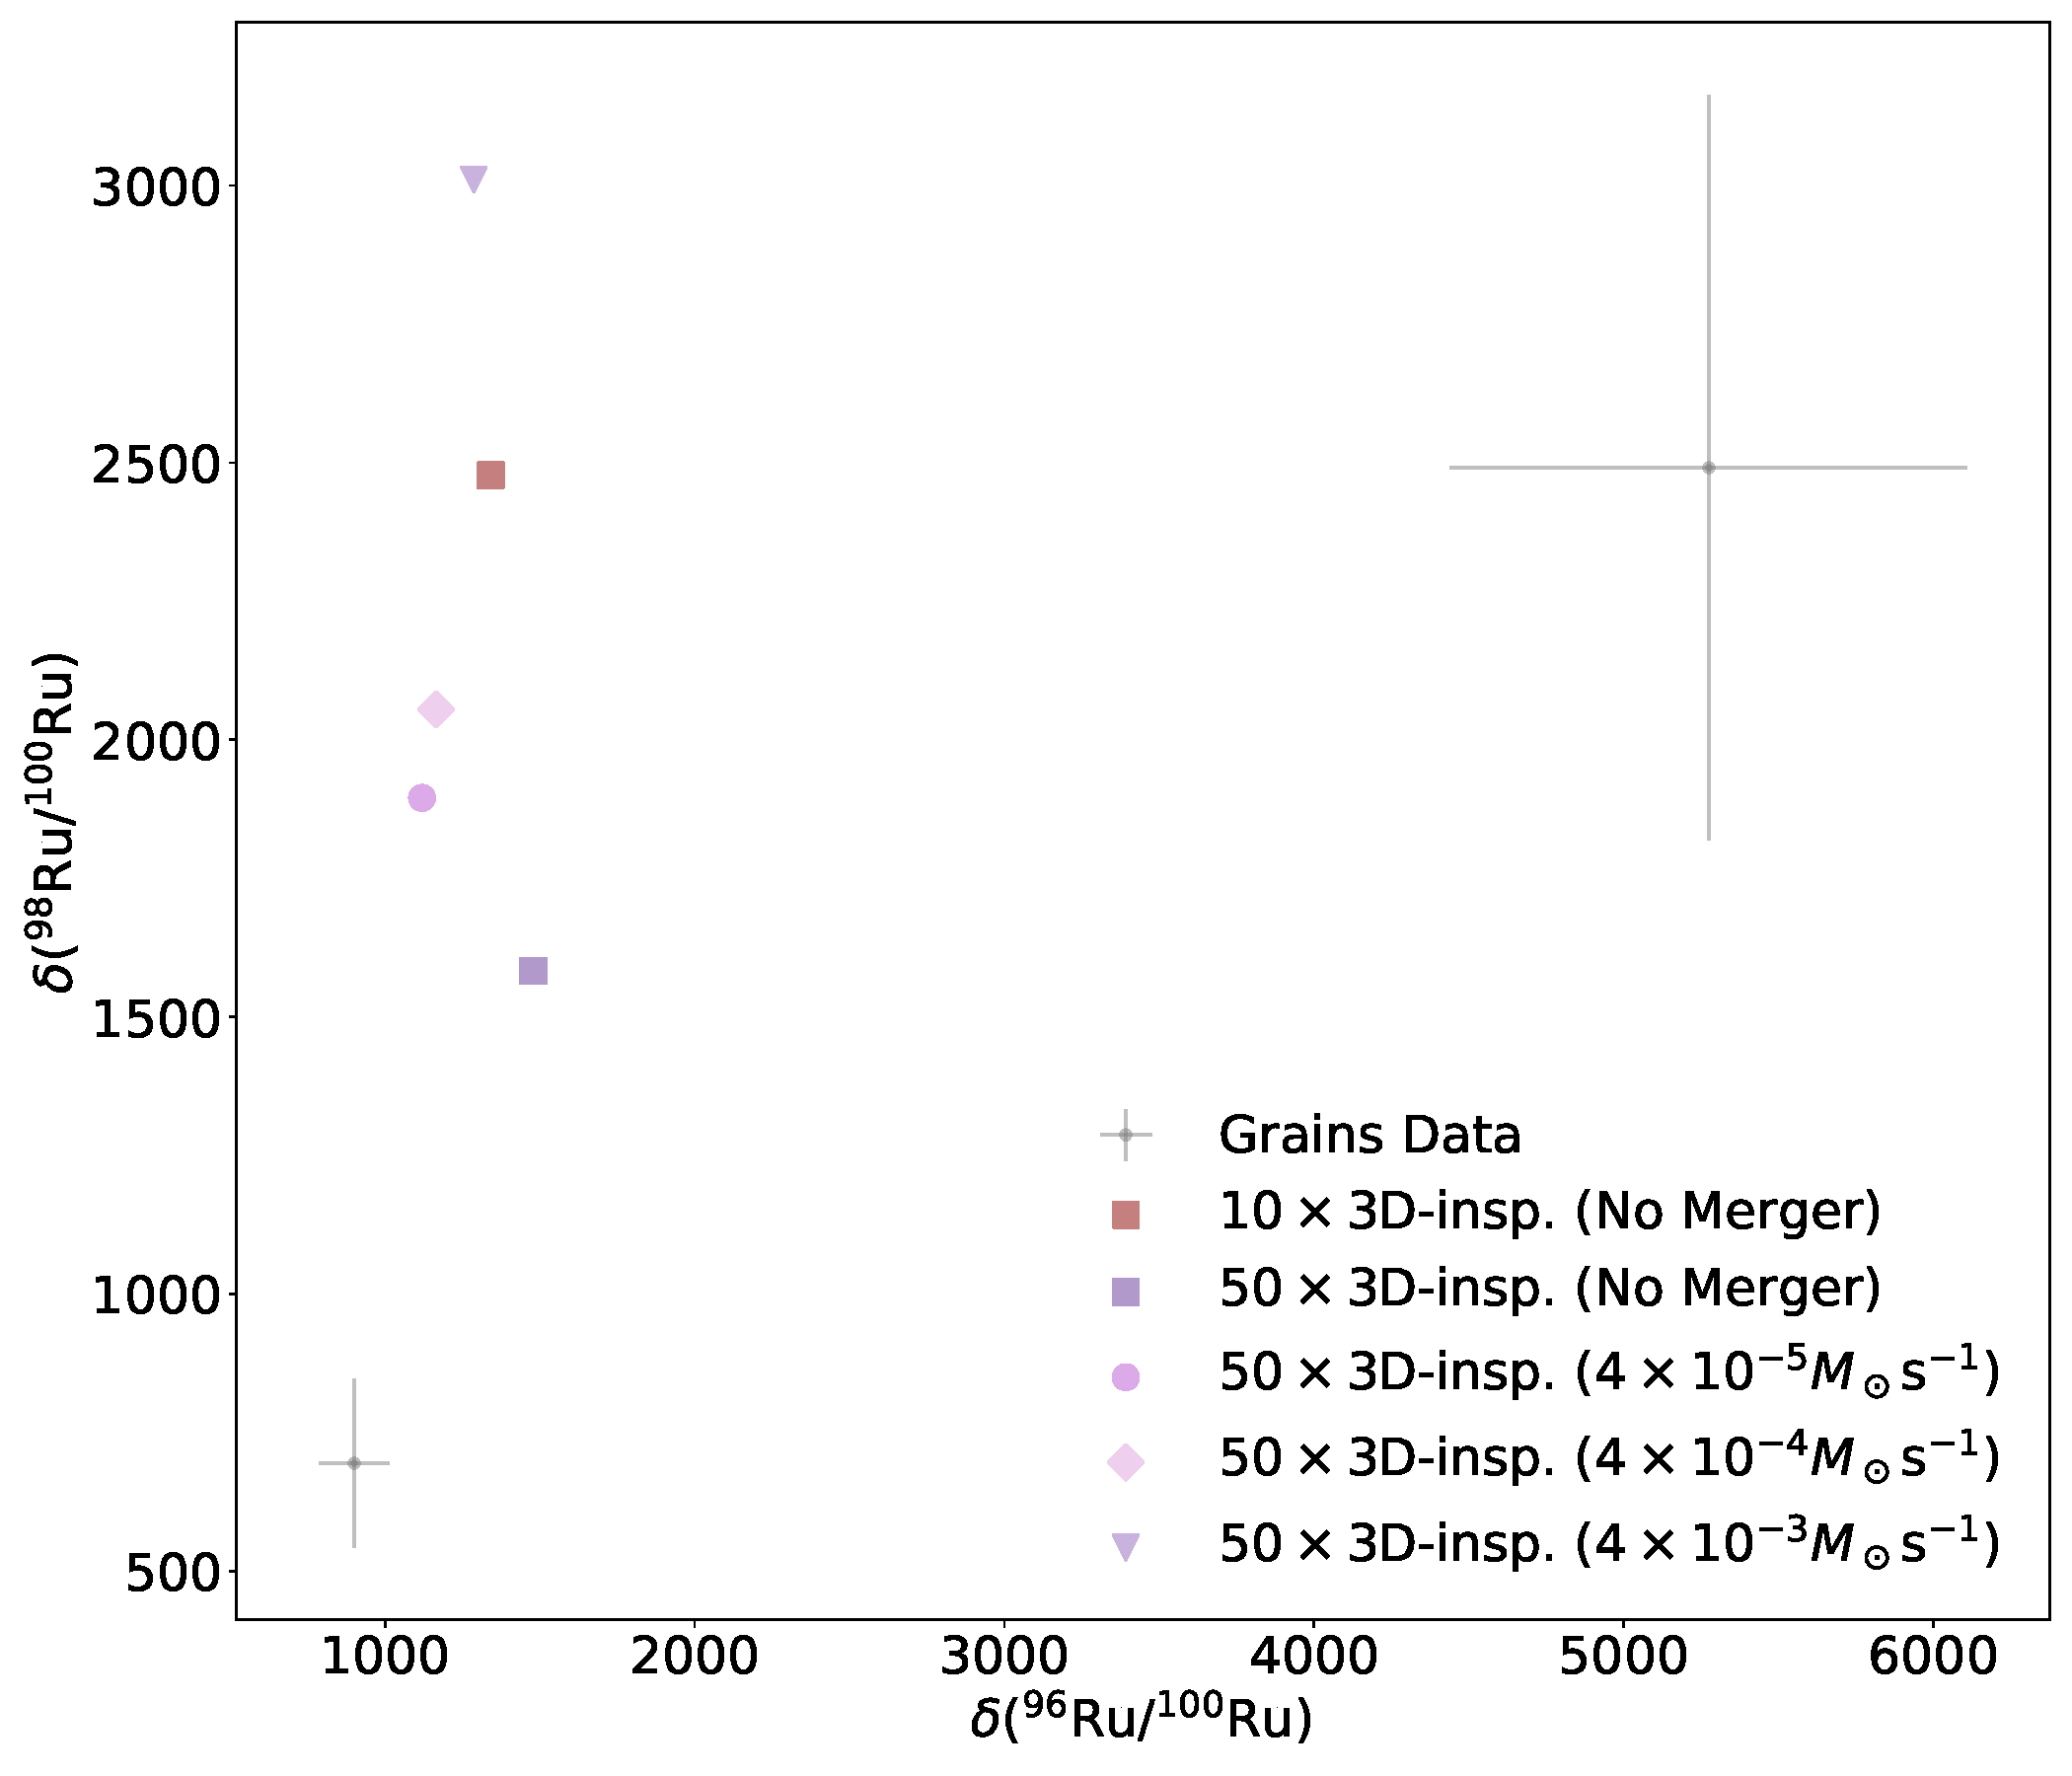
\includegraphics[width=\textwidth]{chapters/2/figures/grains_Ru96_Ru98_Ru100.pdf}
\caption{Comparing the results of the grains data to the various mixing scenarios considered in this paper for $\delta(^{98}\mathrm{Ru}/^{100}\mathrm{Ru})$ and $\delta(^{96}\mathrm{Ru}/^{100}\mathrm{Ru})$. Grey points correspond to grains data with $1\sigma$ error bars and coloured points for the mixing scenarios.
\label{fig:grains_Ru}}
\end{figure}
Figure \ref{fig:grains_Mo} shows that Mo grains can be explained by the 3D-inspired scenario with an ingestion rate of $4\times10^{-3}M_\odot \mathrm{s}^{-1}$ and $4\times10^{-4}M_\odot\mathrm{s}^{-1}$ as well as $3\times$3D-inspired scenario with an ingestion rate of $4\times10^{-3}M_\odot\mathrm{s}^{-1}$ with the MLT, GOSH-like, and partial merger cases close to the measurements.
However, as Figure \ref{fig:grains_Ru} shows, the faster $10\times$ and $50\times$3D-inspired cases better match the Ru grains despite the minimal data.
Additionally, although not shown, the $\delta(^{130}\mathrm{Ba}/^{136}\mathrm{Ba})$ and $\delta(^{132}\mathrm{Ba}/^{136}\mathrm{Ba})$ does not match any mixing scenario.
Although there are limitations to comparing the pre-explosive results from the O-shell alone, it does highlight how grains data can constrain the results of 3-D hydrodynamic simulations.

This work also raises the importance of considering the mixing details in the astrophysical site when providing nuclear reaction rates for experiment proposals.
Whether one identifies a reaction as important to the production of one of the p-nuclei, the strength of that importance, and whether it is a branching pathways leading to a bifurcation in the final distribution are all dependent on the mixing.
This points to the need for greater attention to 1-D stellar modelling as a basis for nuclear physics experimental proposals.

There are limitations to the results in this work and further extentions that could be done. 
We have focused on the impact of mixing and nuclear physics, but there remains open questions about the impact of ingested stable seeds from the C-shell. 
As shown in \cite{travaglioTestingRoleSNe2015} and \cite{battinoHeavyElementsNucleosynthesis2020}, the $s$-, $i$-, and $r$-seeds has an important role in the production of the p-nuclei.
This work shows that the ingestion of the C-shell seeds matter, and that the important reaction pathways depend on mixing speed, but there could be work to identify the specific seeds for each isotope, how that is dependent on mixing case, and if modifications of those seeds via the weak $s$-process earlier in the C-burning shell \citep{pignatariWEAKSPROCESSMASSIVE2010}.
It is also unclear whether the mixing dependency will be seen as strongly in the O-shell mergers of other models that have different temperature profiles and O-shell sizes.
Selection of the NuGrid $15M_\odot$ $Z=0.02$ model could be overemphasizing the impact of these results as of the four NuGrid models with O-C shell mergers it has the largest overproduction factor \citep{ritterConvectivereactiveNucleosynthesisSc2018}, although the other models are $Z=0.01$ and seeds do play a role.
Another open question is how the nucleosynthesis will behave with a dynamic stellar structure as this work holds it static.
There are also some limitations in this work as the \texttt{MPPNP} nuclear network does not include isomeric states which means that  $^{180\mathrm{m}}\mathrm{Ta}$ cannot be produced and it could be that the production mechanisms for $^{113}\mathrm{In}$ and $^{115}\mathrm{Sn}$ are potentially limited \citep{dillmannPProcessSimulationsModified2008}.
Finally, these results are calculated for pre-CCSN conditions and should be run through explosive nucleosynthesis to determine the full impact of O-C shell merger nucleosynthesis as $10-40\%$ of the p-nuclei isotopes occur during explosive nucleosynthesis even with an O-C shell merger \citep{robertiGprocessNucleosynthesisCorecollapse2023}.

\section{Conclusion} \label{sec:conclusion}

This study has demonstrated how O-C shell mergers in massive stars are an astrophysical site for the production of the p-nuclei via the $\gamma$-process.
By analyzing 1-D post-processing nucleosynthesis calculations that incorporate the results of 3-D hydrodynamic simulations, we find that there is significant uncertainty in the production of p-nuclei when considering different mixing scenarios.
We have demonstrated that understanding the mixing details of the O-burning shell are critical that the presence of a convective downturn present a non-linear and non-monotonic effect, how production scales with the rate of ingestion, how dips in the convective profile decrease production, and that the impact that nuclear physics can has is sensitive to mixing details.
This is not to suggest that all of these mixing scenarios are equally likely or could happen, but how the lack of correspondence from 3-D hydrodynamics impacts nucleosynthesis.
Since the O-C shell merger is critical to the nucleosynthesis of a massive star prior to the CCSN regardless of explosive energy \citep{robertiGprocessNucleosynthesisCorecollapse2024b}, we emphasis the importance of these model uncertainties of the mixing scenario of O-shell burning and O-C shell mergers.
